\subsection{Home/Accueil}
\begin{figure}[ht]
    \centering
    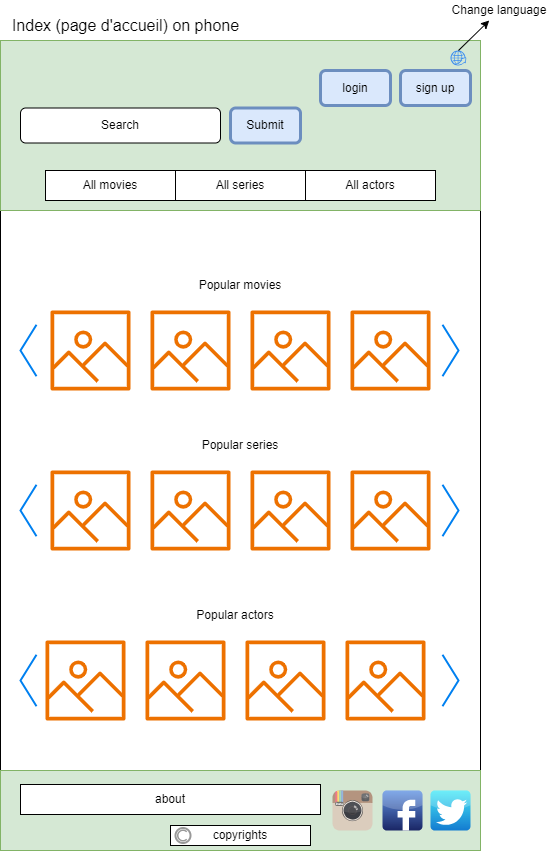
\includegraphics[width=0.8\textwidth, height=0.8\textheight, keepaspectratio]{home/home-tel-not-connected.png}
    \caption{Home page when not connected on phone/Page d'accueil lorsque non connecté sur téléphone}
    \label{fig:home-tel-not-connected}
\end{figure}

\begin{figure}[ht]
    \centering
    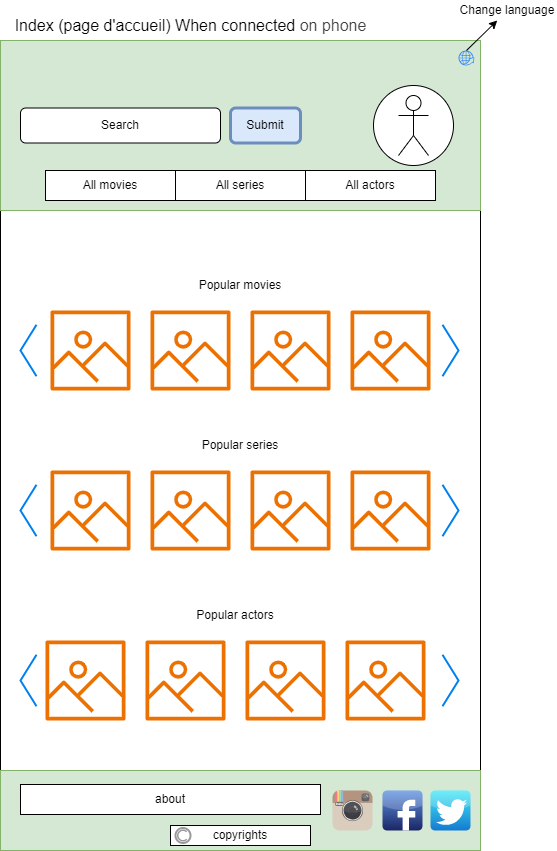
\includegraphics[width=0.8\textwidth, height=0.8\textheight, keepaspectratio]{home/home-tel-connected.png}
    \caption{Home page when connected on phone/Page d'accueil lorsque connecté sur téléphone}
    \label{fig:home-tel-connected}
\end{figure}

\begin{sidewaysfigure}[ht]
    \centering
    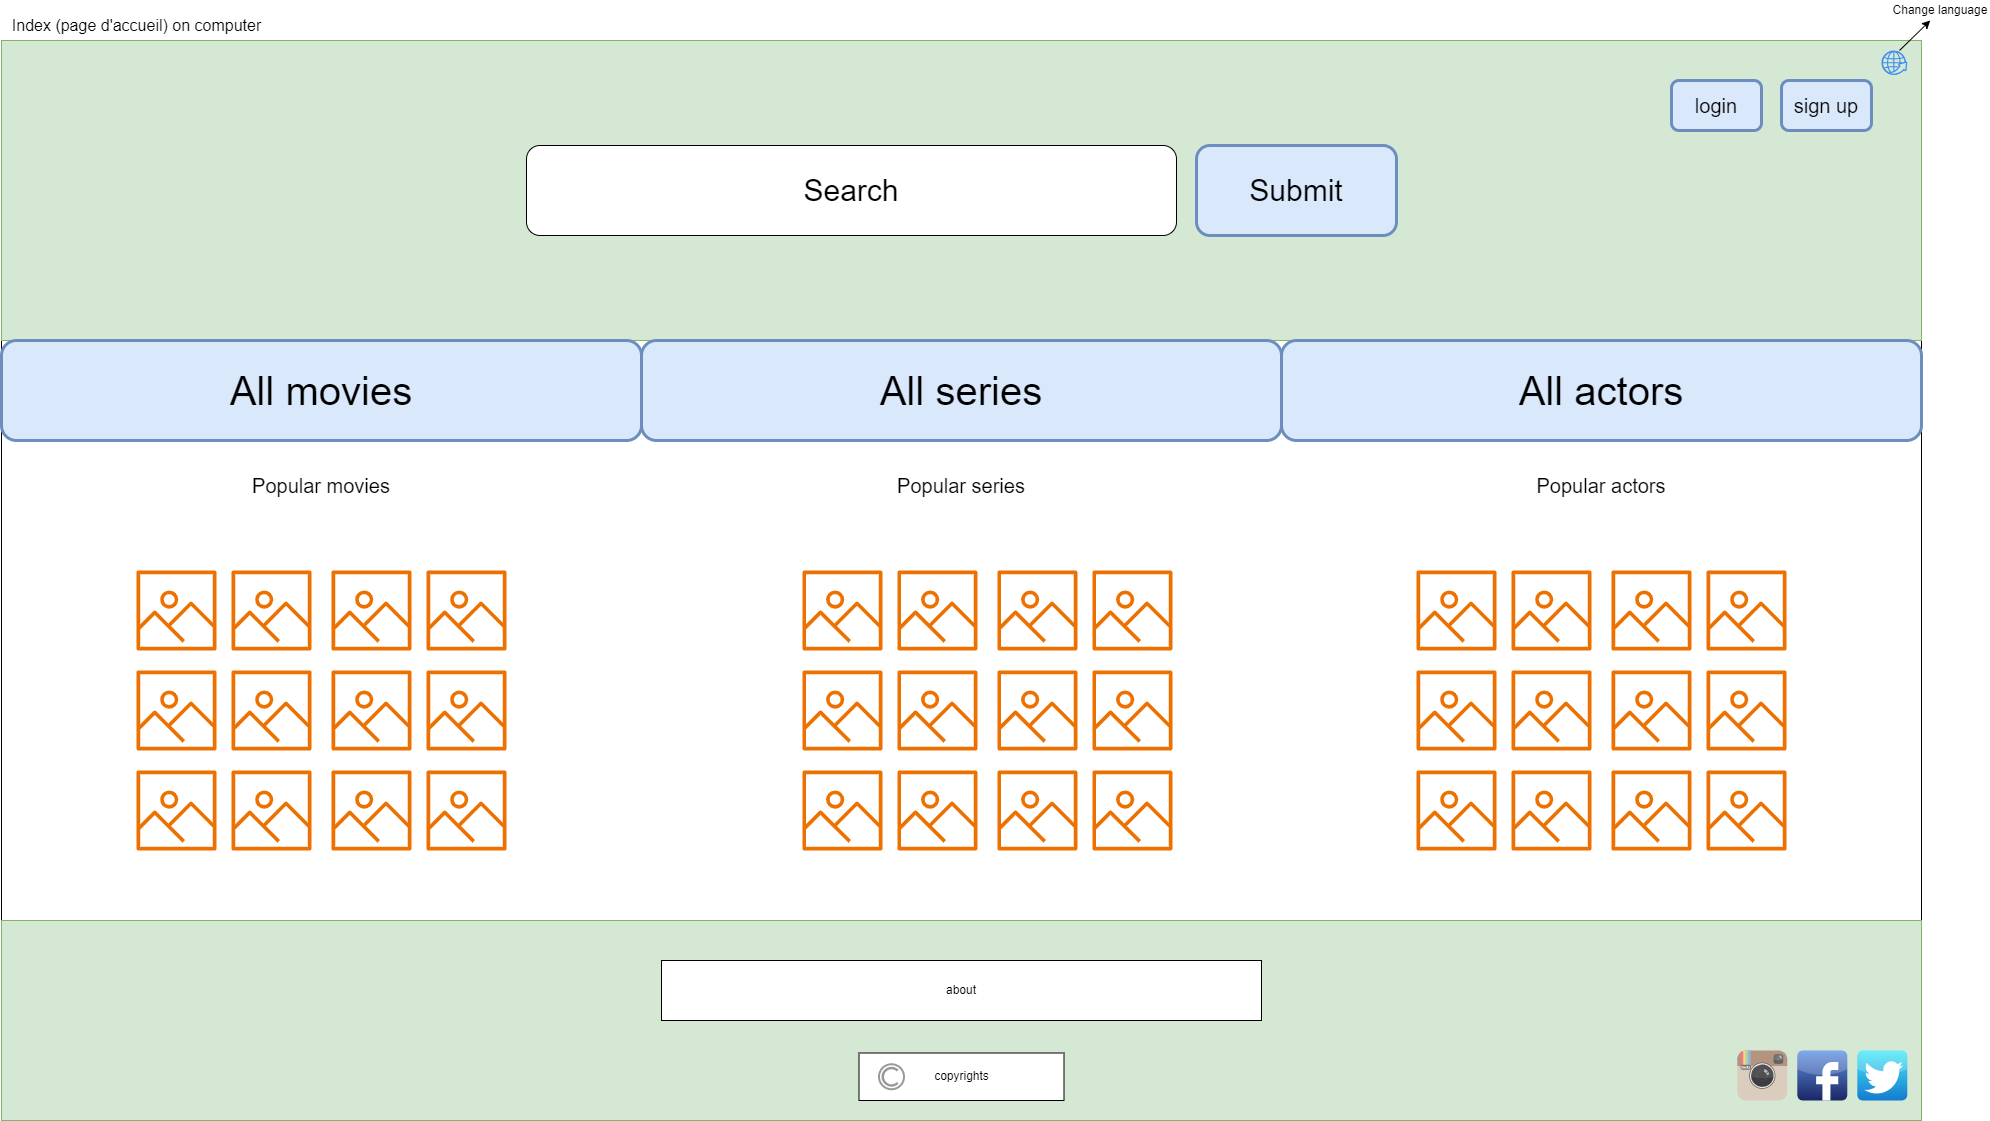
\includegraphics[width=0.8\textwidth, height=0.8\textheight, keepaspectratio]{home/home-comp-not-connected.png}
    \caption{Home page when not connected on computer/Page d'accueil lorsque non connecté sur ordinateur}
    \label{fig:home-comp-not-connected}
\end{sidewaysfigure}

\begin{sidewaysfigure}[ht]
    \centering
    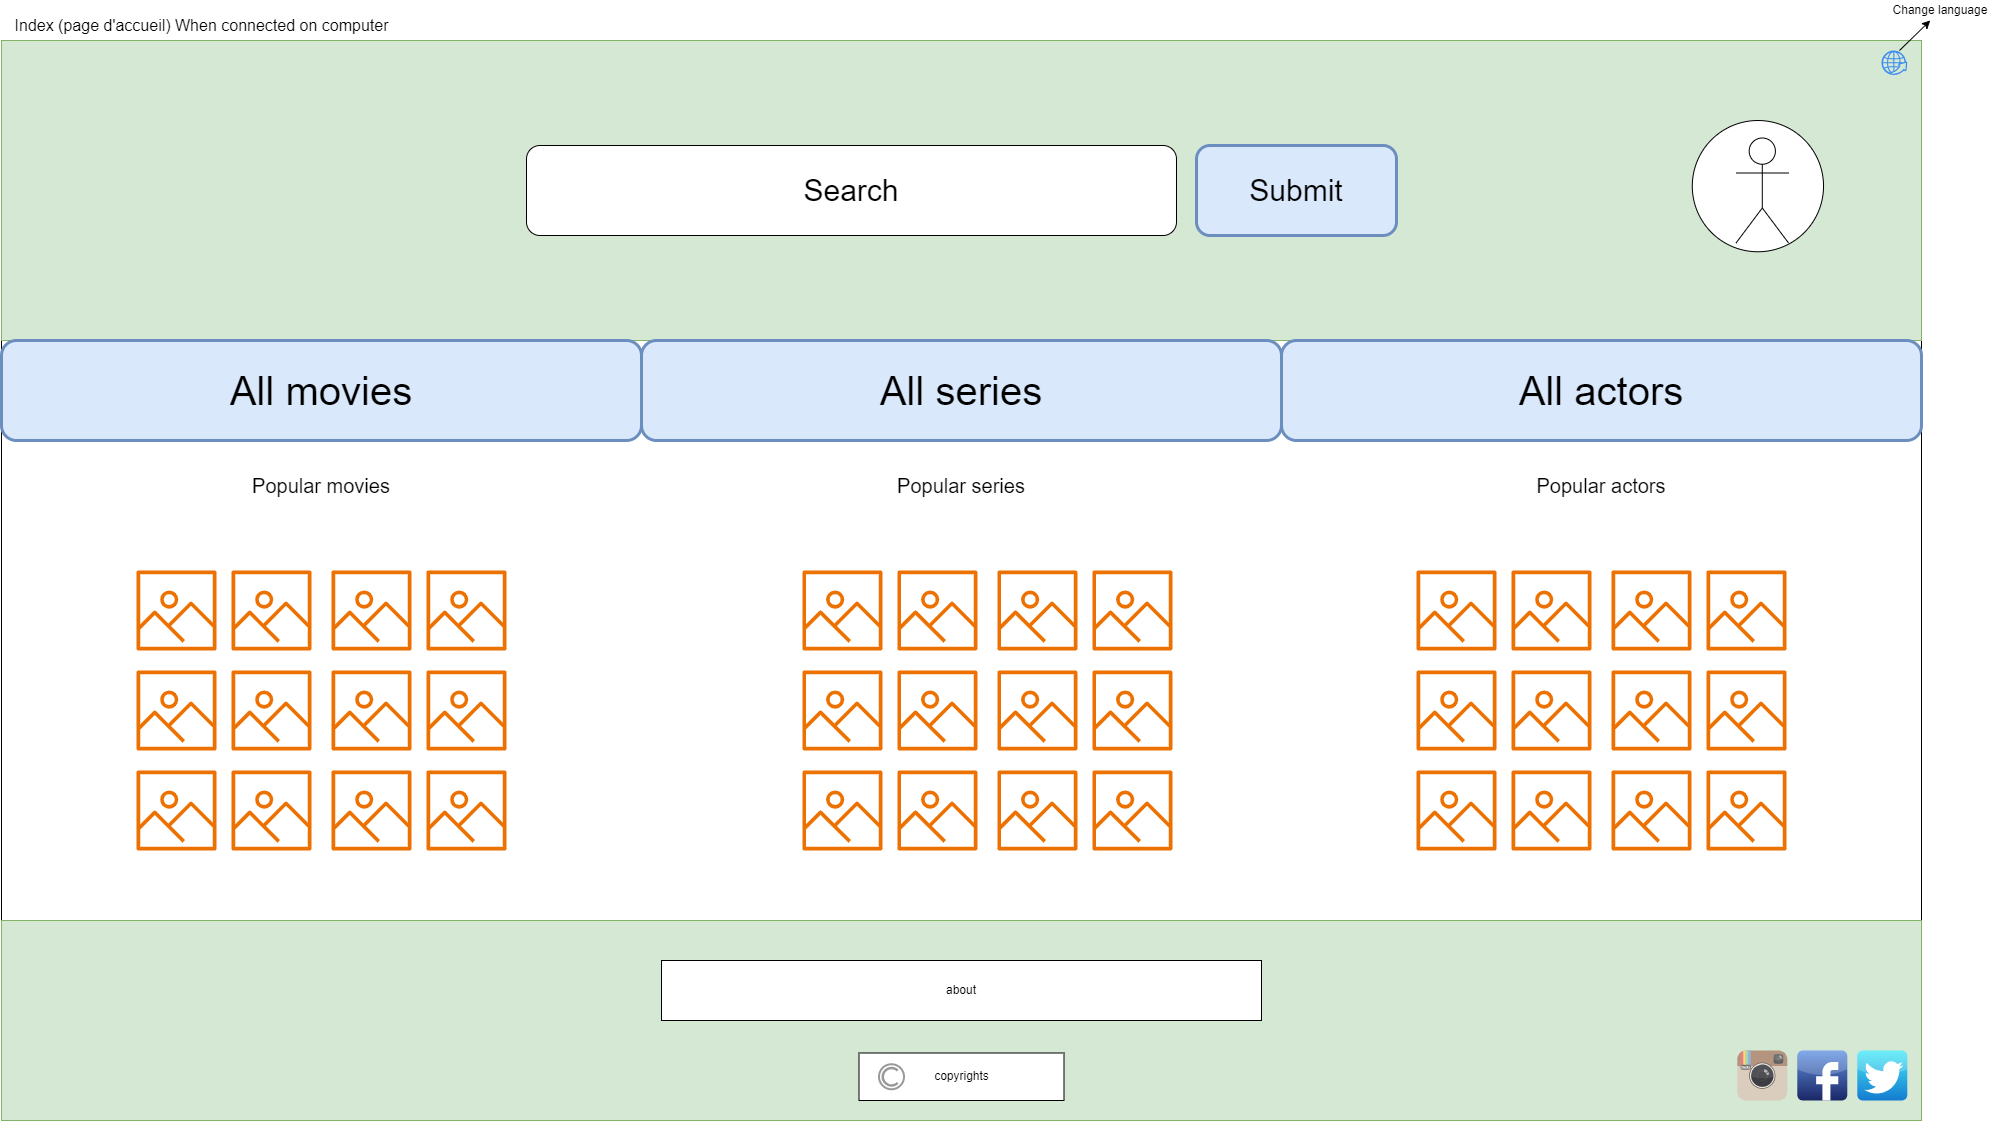
\includegraphics[width=0.8\textwidth, height=0.8\textheight, keepaspectratio]{home/home-comp-connected.png}
    \caption{Home page when connected on computer/Page d'accueil lorsque connecté sur ordinateur}
    \label{fig:home-comp-connected}
\end{sidewaysfigure}

\pagebreak

\subsection{When you click on showing every element/Quand tu clique pour voir tous les éléments}

\begin{sidewaysfigure}[ht]
    \centering
    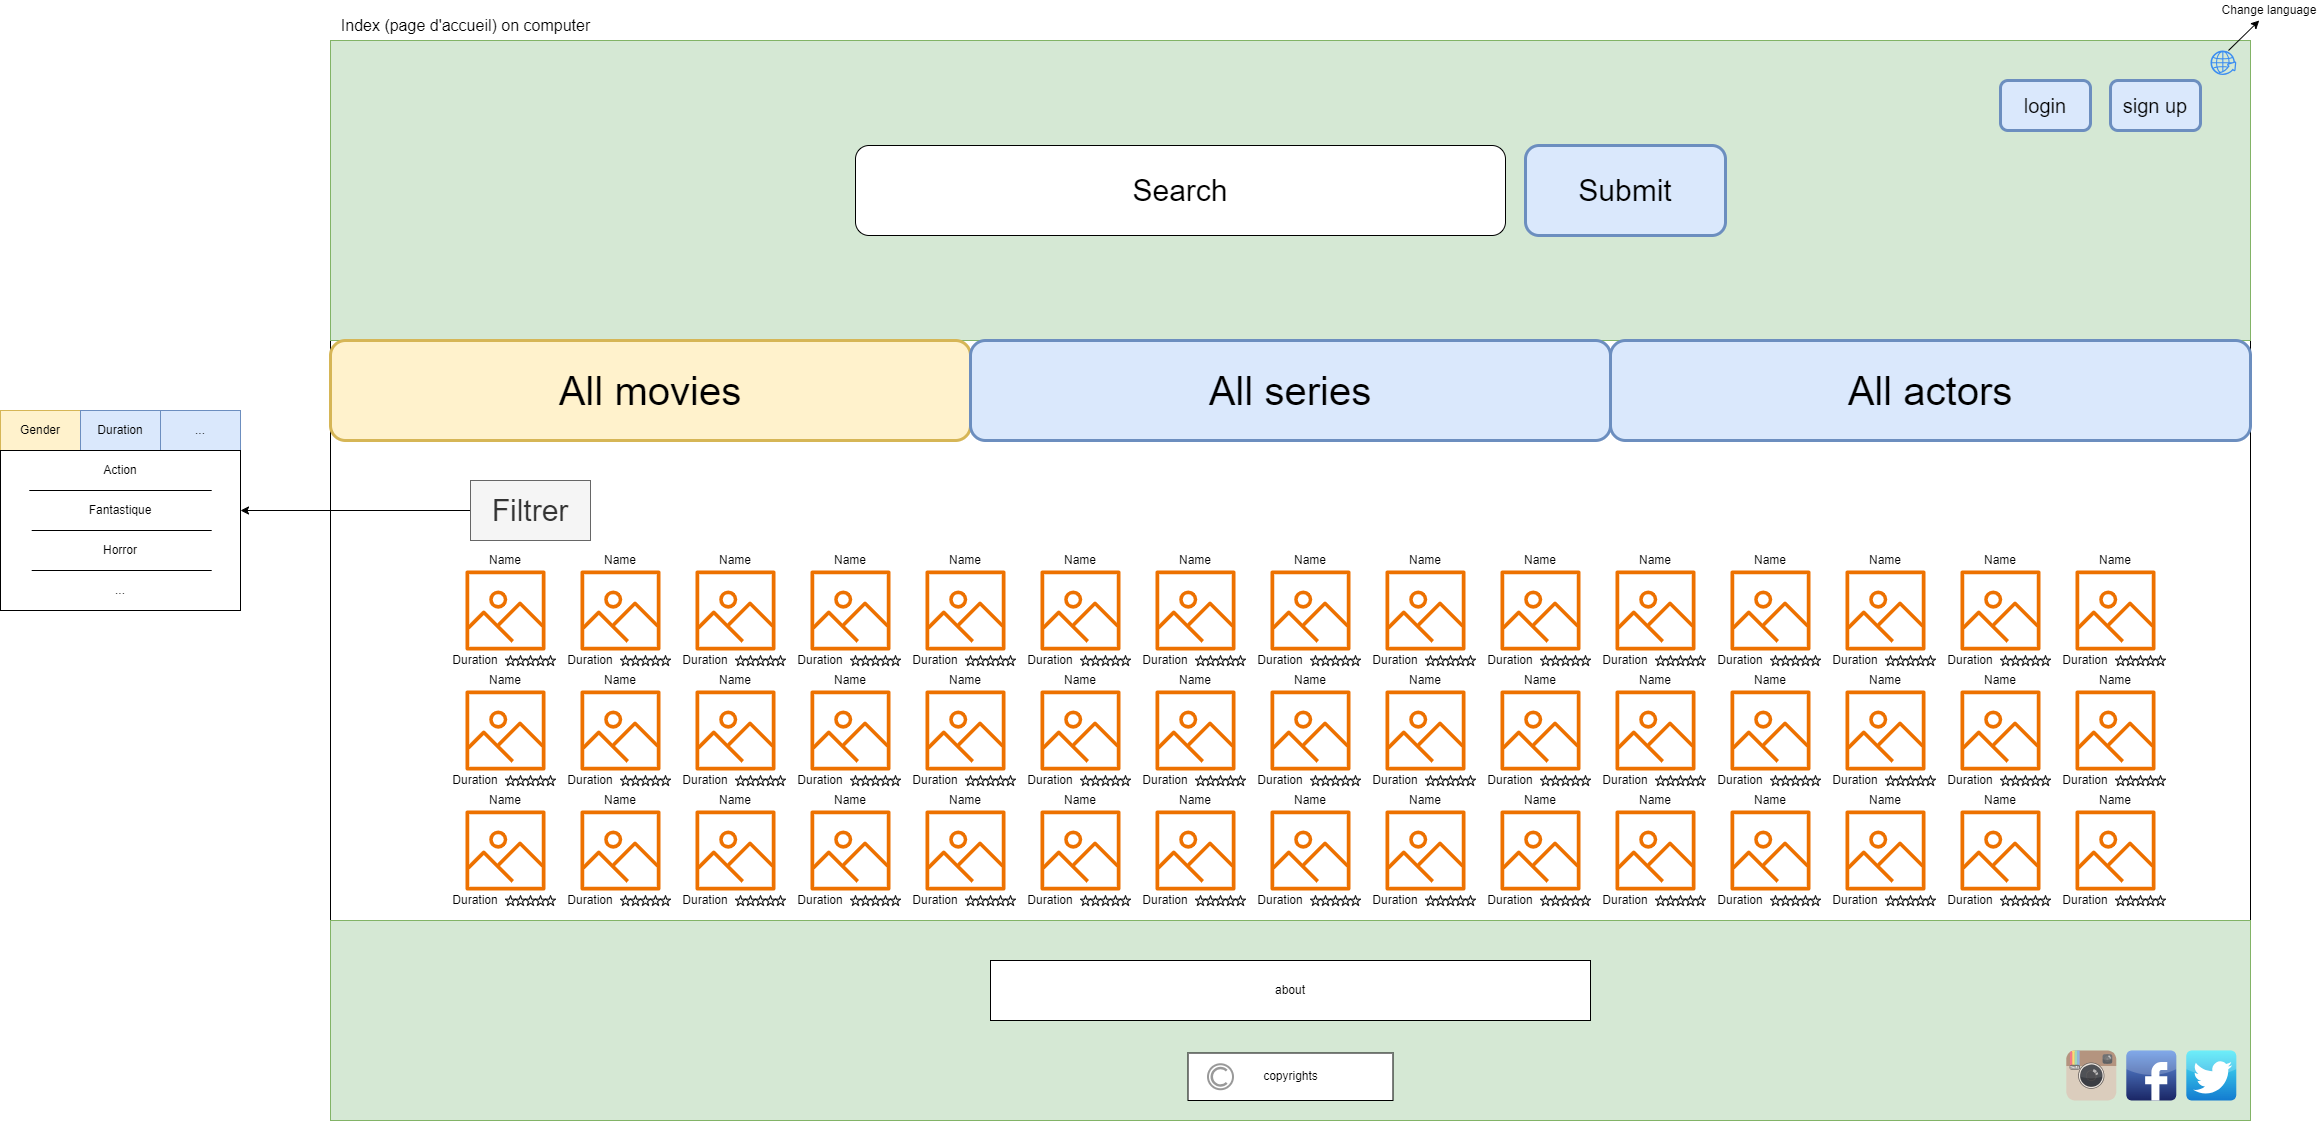
\includegraphics[width=0.8\textwidth, height=0.8\textheight, keepaspectratio]{everything/all-elements.png}
    \caption{Page where you can see every movies or series in one place/Page où vous pouvez voir tous les films ou séries à un seul endroit}
    \label{fig:everything}
\end{sidewaysfigure}

\pagebreak

\subsection{Movies or series informations/Informations sur les films ou séries}

\begin{figure}
    \centering
    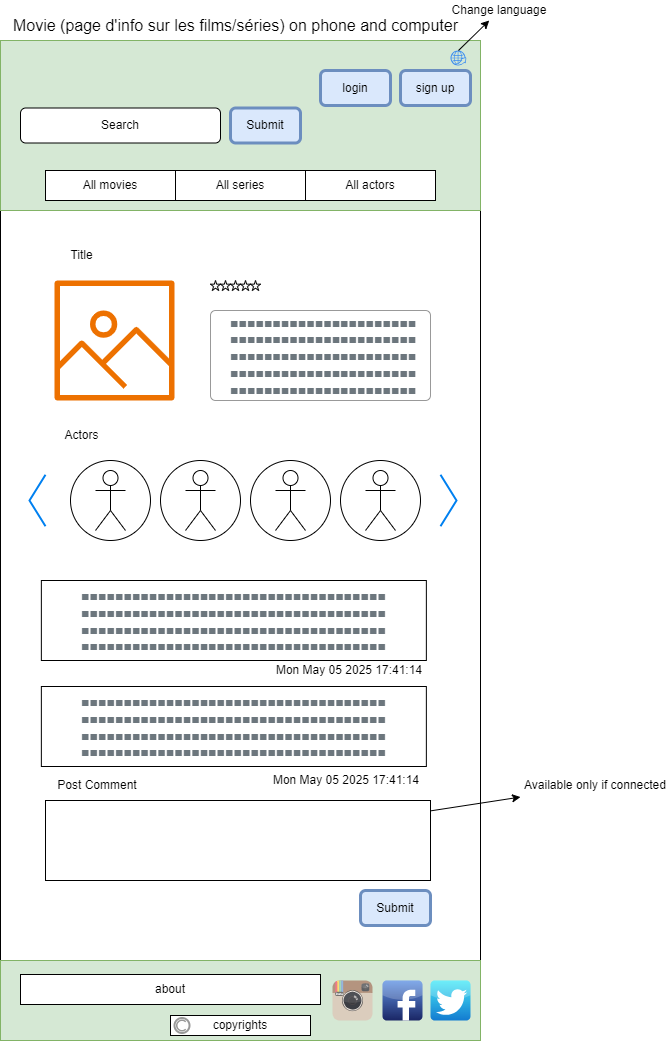
\includegraphics[width=0.8\textwidth, height=0.8\textheight, keepaspectratio]{elem-infos/elem-infos.png}
    \caption{Page where you can see the informations about a movie or a serie/Page où vous pouvez voir les informations à propos d'un film ou d'une série}
    \label{fig:elem-infos}
\end{figure}

\pagebreak

\subsection{User/Utilisateur}

\begin{figure}
    \centering
    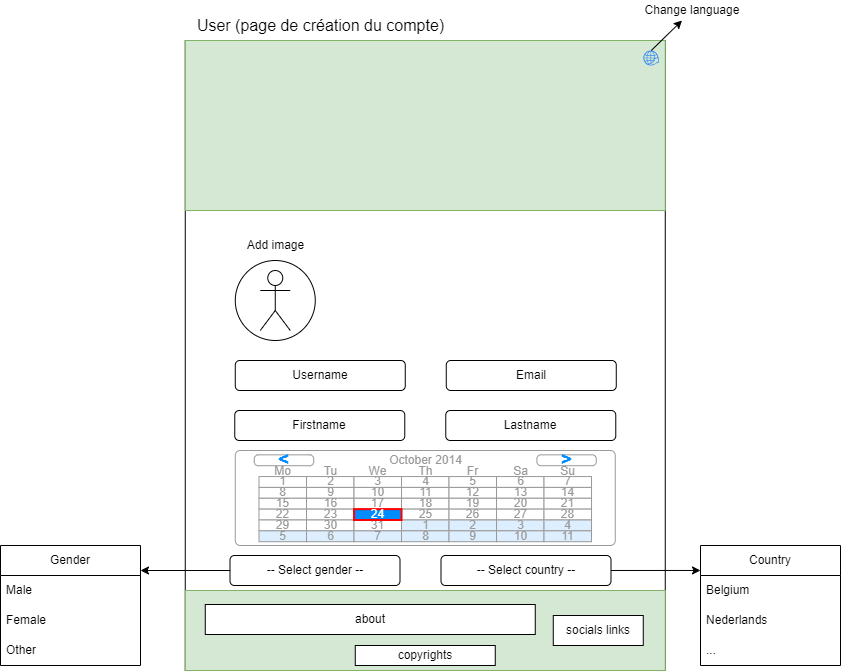
\includegraphics[width=0.8\textwidth, height=0.8\textheight, keepaspectratio]{user/compte-creation.png}
    \caption{Register/Création du compte}
    \label{fig:register}
\end{figure}

\begin{figure}
    \centering
    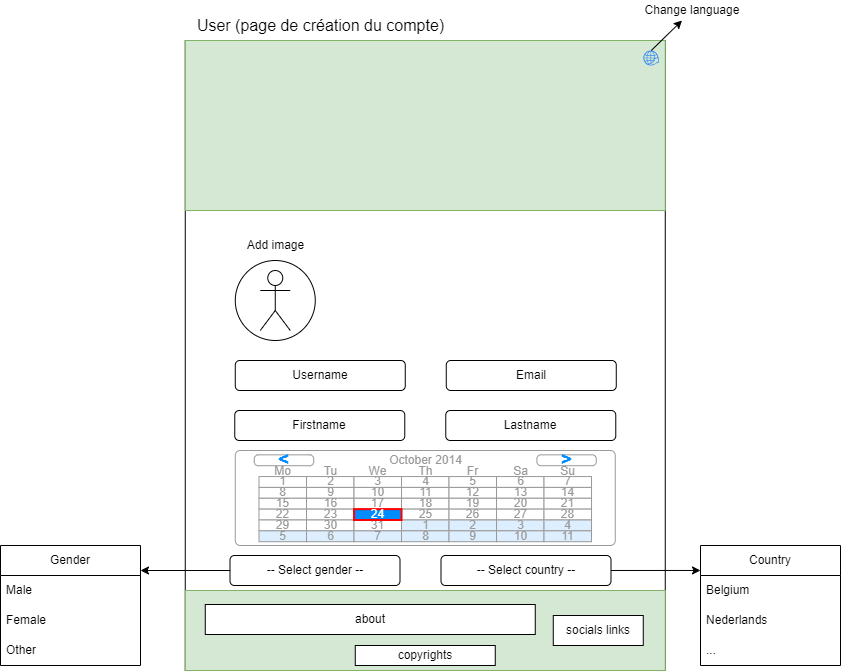
\includegraphics[width=0.8\textwidth, height=0.8\textheight, keepaspectratio]{user/user-infos.png}
    \caption{Page where you can see the user informations/Page où vous pouvez voir les informations à propos d'un utilisateur}
    \label{fig:user-infos}
\end{figure}

\begin{figure}
    \centering
    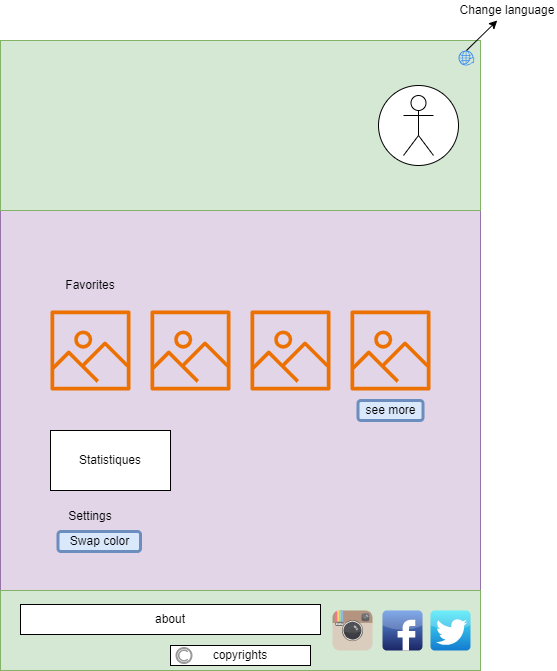
\includegraphics[width=0.8\textwidth, height=0.8\textheight, keepaspectratio]{user/color-change-setting.png}
    \caption{Setting dark mode in action/Paramètre du mode sombre en action}
    \label{fig:color-change-setting}
\end{figure}
